\documentclass{article}

\usepackage[utf8]{inputenc}
\usepackage[T1]{fontenc}
\usepackage{csquotes}
\usepackage[english]{babel}
\usepackage[a4paper, margin=1in]{geometry}
\usepackage[section]{placeins}
\usepackage[backend=biber,maxbibnames=9,sorting=ynt,style=alphabetic]{biblatex}
\usepackage[hidelinks]{hyperref}
\usepackage{appendix}
\usepackage{dutchcal}
\DeclareMathAlphabet{\pazocal}{OMS}{cmsy}{m}{n}
\usepackage{amsmath}
\usepackage{amssymb}
\usepackage{amsthm}
\usepackage{thmtools}
\usepackage{stmaryrd}
\usepackage{mathpartir}
\usepackage{mathtools}
\usepackage{bbm}
\usepackage{xspace}
\usepackage{stackengine}
\usepackage{scalerel}

\usepackage[dvipsnames]{xcolor}
\usepackage{tikz}
\usetikzlibrary{arrows.meta,calc,positioning,shapes.multipart,cd,decorations.pathreplacing}
\usepackage{tikz-cd}
\usepackage{mdframed}
\usepackage[capitalize,noabbrev]{cleveref}

% \usepackage{parskip}  % adds a line between paragraphs

\addbibresource{bibliography.bib}

% Make paragraph bold
\makeatletter
\def\@parfont{\bfseries}
\makeatother

% Shorter section references
\crefformat{section}{\S#2#1#3}

% Removes small-caps font from label in inferrule
\renewcommand{\LabTirName}[1]{{#1}}

% ------------------------
% 1. Misc
% ========================

% Colors and Highlighting.
\colorlet{LightLavender}{Lavender!20!}
\colorlet{Gray}{gray!100!}
\colorlet{LightGray}{gray!40!}
\newcommand{\blue}[1]{\textcolor{blue}{#1}}
\newcommand{\gray}[1]{\textcolor{Gray}{#1}}
\newcommand{\red}[1]{\textcolor{Red}{#1}}
\newcommand{\graym}[1]{\gray{\ensuremath{#1}}}
\newcommand{\note}[1]{\\\red{#1}\\}
\newcommand{\borderedbox}[1]{\fbox{#1}}

\newcommand{\paragraphit}[1]{\noindent\textit{#1.}}

\newcommand{\orpheas}[1]{\red{\textit{Orpheas: }#1}}

% Writing
\newcommand{\eg}{e.g.,\xspace}
\newcommand{\ie}{i.e.,\xspace}
\newcommand{\slab}[1]{\textrm{#1}}

% Spacing
\newcommand{\spac}{\,}

% Other
\def\nop{}
\def\dash{-}

% Tikz Styles for heaplets
\tikzstyle{ptr}=[draw, semithick, {Circle[]}-{Triangle[scale=0.8]}, shorten <=-1mm]
\tikzstyle{dptr}=[draw, semithick, {Circle[]}-{Triangle[scale=0.8]}, shorten <=-1mm, color=red]
\tikzstyle{pricell}=[draw,minimum size=1.6em, outer sep=0pt, label={[shift={(-15pt,-5pt)},color=black]#1}]
\tikzstyle{mpricell}=[draw,minimum size=1.6em, outer sep=0pt, label={[shift={(15pt,-5pt)},color=black]#1}]
\tikzstyle{pubcell}=[draw,minimum size=1.6em, outer sep=0pt, label={[shift={(-15pt,-5pt)},color=blue]#1}]
\tikzstyle{brace}=[draw,decorate,decoration={brace,amplitude=5pt,raise=5ex}]
\tikzstyle{labbrace}=[midway,xshift=3.5em,yshift=1pt]
\tikzstyle{mbrace}=[draw,decorate,decoration={brace,amplitude=5pt,mirror,raise=6ex}]
\tikzstyle{lambrace}=[midway,xshift=-4em]

% Tikz arrow movements
\def\north{(0,0.55)}
\def\west{(-0.5,0)}
\def\wwest{(-0.75,0)}
\def\east{(0.5,0)}
\def\eeast{(0.75,0)}
\def\south{(0,-0.55)}

% ------------------------
% 2. Mathematics.
% ========================

% Misc
\newcommand{\eqdef}{:=}
\newcommand{\inddef}{::=}
\newcommand{\where}{\;\mathit{where}\;}
\def\iso{\cong}
\newcommand{\img}[1]{\mathsf{Im}(#1)}
\newcommand{\inv}[1]{{#1}^{-1}}
\renewcommand{\vec}{\overline}
\def\xto{\xrightarrow}
\def\injto{\rightarrowtail}
\def\inclto{\hookrightarrow}
\def\xinclto{\xhookrightarrow}
\def\surjo{\twoheadrightarrow}
\def\bito{\leftrightarrow}
\newcommand{\minfun}{\mathsf{min}\spac}
\newcommand{\Succ}{\mathit{S}\,}
\newcommand{\Proof}{\noindent\textit{Proof:}\;}
\newcommand{\suchthat}{\textit{s.t.}}
\newcommand{\syntax}[1]{\;\ulcorner{\hspace{-1pt}#1\hspace{-1pt}}\urcorner\;}

% Term list.
\newcommand{\tlist}[2]{{#1}_1,...,{#1}_{#2}}
\newcommand{\tlistr}[2]{(#1)_{#2}}
\newcommand{\tsetr}[2]{\{#1\}_{#2}}

% Common metavariables.
% -- Vectors of binders.
\newcommand{\vxs}{\vec\x}
\newcommand{\vys}{\vec\y}
% -- Variables.
\newcommand{\va}{\mathit{a}}
\newcommand{\vb}{\mathit{b}}
\newcommand{\vc}{\mathit{c}}
\newcommand{\vd}{\mathit{d}}
\newcommand{\ve}{\mathit{e}}
\newcommand{\vf}{\mathit{f}}
\newcommand{\vg}{\mathit{g}}
\newcommand{\vh}{\mathit{h}}
\newcommand{\vi}{\mathit{i}}
\newcommand{\vj}{\mathit{j}}
\newcommand{\vk}{\mathit{k}}
\newcommand{\vl}{\mathit{l}}
\newcommand{\vm}{\mathit{m}}
\newcommand{\vn}{\mathit{n}}
\newcommand{\vo}{\mathit{o}}
\newcommand{\vp}{\mathit{p}}
\newcommand{\vq}{\mathit{q}}
\newcommand{\vr}{\mathit{r}}
\newcommand{\vs}{\mathit{s}}
\newcommand{\vt}{\mathit{t}}
\newcommand{\vu}{\mathit{u}}
\newcommand{\vv}{\mathit{v}}
\newcommand{\vw}{\mathit{w}}
\newcommand{\vx}{\mathit{x}}
\newcommand{\vy}{\mathit{y}}
\newcommand{\vz}{\mathit{z}}
\newcommand{\vA}{\mathit{A}}
\newcommand{\vB}{\mathit{B}}
\newcommand{\vC}{\mathit{C}}
\newcommand{\vD}{\mathit{D}}
\newcommand{\vE}{\mathit{E}}
\newcommand{\vF}{\mathit{F}}
\newcommand{\vG}{\mathit{G}}
\newcommand{\vH}{\mathit{H}}
\newcommand{\vI}{\mathit{I}}
\newcommand{\vJ}{\mathit{J}}
\newcommand{\vK}{\mathit{K}}
\newcommand{\vL}{\mathit{L}}
\newcommand{\vM}{\mathit{M}}
\newcommand{\vN}{\mathit{N}}
\newcommand{\vO}{\mathit{O}}
\newcommand{\vP}{\mathit{P}}
\newcommand{\vQ}{\mathit{Q}}
\newcommand{\vR}{\mathit{R}}
\newcommand{\vS}{\mathit{S}}
\newcommand{\vT}{\mathit{T}}
\newcommand{\vU}{\mathit{U}}
\newcommand{\vV}{\mathit{V}}
\newcommand{\vW}{\mathit{W}}
\newcommand{\vX}{\mathit{X}}
\newcommand{\vY}{\mathit{Y}}
\newcommand{\vZ}{\mathit{Z}}
% Conventional metavariables.
\newcommand{\var}{\mathit{x}}
\newcommand{\Var}{\mathit{X}}
\newcommand{\val}{\mathit{V}}
\newcommand{\wal}{\mathit{W}}
\newcommand{\vop}{\mathit{op}}
\newcommand{\compM}{\mathit{M}}
\newcommand{\compN}{\mathit{N}}
\newcommand{\pvarA}{\mathit{a}}
\newcommand{\pvarB}{\mathit{b}}
\newcommand{\pvarC}{\mathit{c}}
\newcommand{\pvarD}{\mathit{d}}
\newcommand{\ubar}[1]{\hat{#1}}

% Maps.
\newcommand{\mapbinding}{\mapsto}
\newcommand{\mapempty}{\varnothing}
\newcommand{\maplookup}[2]{#1(#2)}
\newcommand{\mapupdate}[2]{[{#1} \mapbinding {#2}]}
\newcommand{\Dom}[1]{\mathit{Dom}(#1)}

% Lists.
\newcommand{\concatOp}{+\hspace{-4pt}+\spac}
\newcommand{\listCons}{;}
\newcommand{\listSing}[1]{[#1]}
\newcommand{\listTwo}[2]{[#1; #2]}
\newcommand{\listApp}{\concatOp}
\newcommand{\listNil}{[]}
\newcommand{\card}[1]{|#1|}

% Sets
\newcommand{\singSet}[1]{\{ #1 \}}
\newcommand{\emptySet}{\emptyset}
\newcommand{\powerSet}[1]{\mathcal{P}(#1)}
\newcommand{\terminalSet}{\singSet{*}}
\newcommand{\downsetsml}[1]{{#1\downarrow}}
\newcommand{\downset}[1]{{#1\hspace{-2pt}\downarrow}}
\newcommand{\setDiff}{\setminus}

% -----------------------------------
% 3. Parametrised Algebraic theories.
% ===================================

\newcommand{\algtyped}[3]{#1 \vdash #2 : #3}
\newcommand{\algeqtyped}[3]{#1 \vdash #2 \equiv #3}
\newcommand{\ptyped}[3]{#1 \mid #2 \vdash #3}
\newcommand{\peqtyped}[4]{#1 \mid #2 \vdash & #3 \equiv #4}

\newcommand{\sorts}[1]{\underbar{$#1$}_{\mathsf{s}}}
\newcommand{\supp}[1]{\underbar{$#1$}}
\newcommand{\MatchContSing}[2]{\kw{match}\spac #1 \To\spac #2 }
\newcommand{\MatchCont}[4]{\kw{match}\spac #1 \To\spac #2 ; #3 \To\spac #4}
\newcommand{\MatchContVec}[2]{\kw{match}\spac \{ #2 \}_{#1}}
\newcommand{\MatchContVert}[4]{
\begin{array}[t]{@{}l}
    \kw{match} \\
    \quad #1 \To \spac #2; \\
    \quad #3 \To \spac #4
\end{array}}
\newcommand{\MatchContThreeVert}[6]{
    \begin{array}[t]{@{}l}
    \kw{match} \\
    \quad #1 \To \spac #2; \\
    \quad #3 \To \spac #4; \\
    \quad #5 \To \spac #6
\end{array}}

\def\Mod{\mathfrak{M}}
\def\Param{\mathfrak{p}}

\def\eqOp{\ensuremath{?_=}}
\newcommand{\eqOpArg}[2]{?_{#1 = #2}}
\def\eqOpVerb{\mathit{eq}}
\def\newOp{\ensuremath{\nu}}
\def\readOp{\mathit{r}}
\def\writeOp{\mathit{w}}
\def\newOpMA{\newOp_{\triple{\vw_1}{\vw_2}{\vh}}}
\def\newOpMB{\newOp_{\triple{\vw_1'}{\vw_2'}{\vh'}}}
\def\newOpME{\newOp_{\triple\listNil\listNil\mapempty}}
\def\writeOpMA{\writeOp^\vC_{\tup{\vw}{\vd}}}
\def\writeOpMB{\writeOp^\vC_{\tup{\vw'}{\vd'}}}
\def\writeOpMC{\writeOp^\vC_{\tup{\vw_1}{\vd_1}}}
\def\writeOpMD{\writeOp^\vC_{\tup{\vw_2}{\vd_2}}}
\newcommand{\eqTerm}[4]{#3 \,?_{#1 = #2}\, #4}
\newcommand{\eqTermVerb}[4]{\eqOpVerb(#1, #2, #3, #4)}
\newcommand{\newTerm}[2]{\newOp_{#1}{#2}.\spac}
\newcommand{\readTerm}[3]{\readOp(#1, #2, #3)}
\newcommand{\writeTerm}[3]{\writeOp_{#1}(#2, #3)}

% ------------------------
% 4. Programming Language.
% ========================

\newcommand{\kw}[1]{{\rm {\bf #1}}}
\newcommand{\weaken}[2]{\prescript{#1}{}{\hspace{-1pt}#2}}

\def\colLinkedList{\mathrm{linked\_list}}
\def\colData{\mathrm{data}}
\def\lamref{\lambda_\mathsf{ref}}

% Identifiers.
\newcommand{\ident}[1]{\ensuremath{\mathit{#1}}\xspace}
% Abstraction.
\newcommand{\Lam}[1]{\lambda#1.\spac}
\newcommand{\LamT}[2]{\lambda(#1 \,: #2).\spac}
\newcommand{\LamTwo}[2]{\lambda#1\spac#2.\spac}
\newcommand{\LamTwoT}[4]{\lambda(#1 \spac: #2)\spac(#3 \spac: #4).\spac}
\newcommand{\LamThree}[3]{\lambda#1\spac#2\spac#3.\spac}
\newcommand{\LamFour}[4]{\lambda#1\spac#2\spac#3\spac#4.\spac}
% Application.
\newcommand{\App}{\spac}
\newcommand{\BApp}[1]{(#1)}
% Return
\newcommand{\Ret}{\kw{return}\spac}
% Do
\newcommand{\revto}{\leftarrow}
\newcommand{\Do}[2]{\kw{do}\spac\mathit{#1}\revto{#2}\spac\kw{in}\spac}
\newcommand{\DoT}[3]{\kw{do}\spac(\mathit{#1} : #2)\revto{#3}\spac\kw{in}\spac}
\newcommand{\DoInVertical}[3]{
\begin{array}[t]{@{}l}
    \kw{do}\spac\mathit{#1}\revto{#2}\spac\kw{in}                                \\
    #3
\end{array}}
\newcommand{\DoVerticalIn}[3]{
\begin{array}[t]{@{}l}
    \kw{do}\spac\mathit{#1}\revto{#2}                                            \\
    \kw{in}\spac{#3}
\end{array}}
% Thunks
\newcommand{\Thunk}{\kw{thunk}\spac}
\newcommand{\Force}{\kw{force}\spac}
% Operation Call
\newcommand{\OCall}[3]{{#1}\BApp{{#2};{#3}}}
\newcommand{\Kont}[1]{{#1}.}
% If-Then
\newcommand{\IfThenElse}[2]{\kw{if}\spac{#1}\spac\kw{then}\spac{#2}\spac\kw{else}\spac}
% Pairs
\newcommand{\Unit}{()}
\newcommand{\VPair}[2]{( #1 , #2 )}
\newcommand{\Pair}[2]{\langle #1 , #2 \rangle}
\newcommand{\Fst}{\kw{fst}\spac}
\newcommand{\Snd}{\kw{snd}\spac}
\newcommand{\Split}[3]{\kw{split}\spac{#1}\spac\kw{as}\spac\Pair{#2}{#3}.\spac}
\newcommand{\SplitVertical}[4]{
\begin{array}[t]{@{}l}
\kw{split}\spac{#1}\spac\{ \\
    \qquad \Pair{#2}{#3}. \spac #4 \\
\}
\end{array}}
% Variants
\newcommand{\InjL}{\kw{inl}\spac}
\newcommand{\InjR}{\kw{inr}\spac}
\newcommand{\Case}[5]{\kw{case}\spac{#1}\spac\{ #2.\spac #3 ; #4. \space #5 \}}
\newcommand{\CaseVertical}[5]{
\begin{array}[t]{@{}l}
    \kw{case}\spac{#1}\spac \\
    \quad#2. \spac #3 \\
    \quad#4. \spac #5
\end{array}}
\newcommand{\Absurd}[1]{\kw{case}\spac{#1}\{\}}

% ------------------------
% 5. Types.
% ========================

% Keywords.
\newcommand{\typekw}[1]{\textsf{#1}}

% Programming-language Kinds.
\newcommand{\Type}{\mathsf{Type}}
\newcommand{\Comp}{\mathsf{Comp}}
\newcommand{\Signature}{\mathsf{Signature}}

% Kind variables
\newcommand{\kvarK}{\kappa}

% Type variables
\newcommand{\tvarA}{\alpha}
\newcommand{\tkvarA}[1]{\tvarA^{#1}}
\newcommand{\tvarB}{\beta}
\newcommand{\tvarC}{\gamma}
\newcommand{\tkvarC}[1]{\tvarC^{#1}}
\newcommand{\tvarsA}{\vec\alpha}

% Kind metavariables
\newcommand{\kmvarK}{K}
\newcommand{\kmvarP}{\hat\kmvarK}

% Value type metavariables
\newcommand{\vtmvarA}{A}
\newcommand{\vtmvarB}{B}
\newcommand{\vtmvarC}{C}
\newcommand{\vtmvarD}{D}

% Computation type metavariables
\newcommand{\ctype}[1]{\underline{\textnormal{#1}}}
\newcommand{\ctmvarA}{\ctype\vtmvarA}
\newcommand{\ctmvarB}{\ctype\vtmvarB}
\newcommand{\ctmvarC}{\ctype\vtmvarC}
\newcommand{\ctmvarD}{\ctype\vtmvarD}

\newcommand{\tmvarT}{T}

% Signature meta-variables
\newcommand{\smvarS}{\Sigma}
\newcommand{\smvarT}{\smvarS'}

% Signatures
\newcommand{\sig}{\mid}
\newcommand{\sigNil}{\cdot}
\newcommand{\sigPlus}{\uplus}

% Value types
\newcommand{\tyZ}{\typekw{0}}
\newcommand{\tyUnit}{\typekw{1}}
\newcommand{\tyBool}{\typekw{B}}
\newcommand{\tyNat}{\typekw{N}}
\newcommand{\tyRef}[1]{\typekw{ref}_{#1}}
\newcommand{\tyParam}{\pi}
\newcommand{\tyU}{\typekw{U}\spac}
\newcommand{\tySum}{\spac\typekw{$+$}\spac}
\newcommand{\tyProd}{\spac\typekw{$\times$}\spac}

% Computation types
\newcommand{\tyF}{\typekw{F}}
\newcommand{\tyFun}{\rightarrow}
\newcommand{\tyCProd}{\spac\typekw{$\&$}\spac}

% ------------------------
% 6. Typing Judgments
% ========================

\newcommand{\parctx}{\Delta}
\newcommand{\parctxB}{\parctx'}
\newcommand{\valctx}{\Gamma}
\newcommand{\valctxB}{\valctx'}
\newcommand{\ctxPlus}{+}
\newcommand{\ctxNil}{\cdot}

\newcommand{\Vars}[1]{\mathsf{Var}\spac#1}
\newcommand{\FVars}[1]{\mathsf{FreeVar}\spac#1}

\newcommand{\ctyped}[4]{#1 \mid #2 \vdash_{\mathsf{c}} #3 : #4}
\newcommand{\vtyped}[4]{#1 \mid #2 \vdash_{\mathsf{v}} #3 : #4}
\newcommand{\eqtyped}[5]{#1 \mid #2 \vdash_{\mathsf{c}} #3 = #4 : #5}

\newcommand{\RULEDEF}[2]{\hypertarget{#1}{{(#2)}}\xspace}
\newcommand{\RULE}[2]{\hyperlink{#1}{(#2)}\xspace}

\newcommand{\nameTVar}{T-Var}
\newcommand{\nameTThunk}{T-Thunk}
\newcommand{\nameTInjL}{T-Injl}
\newcommand{\nameTInjR}{T-Injr}
\newcommand{\nameTUnit}{T-Unit}
\newcommand{\nameTVPair}{T-VPair}
\newcommand{\nameTApp}{T-App}
\newcommand{\nameTLam}{T-Lam}
\newcommand{\nameTForce}{T-Force}
\newcommand{\nameTReturn}{T-Ret}
\newcommand{\nameTDo}{T-Do}
\newcommand{\nameTPair}{T-Pair}
\newcommand{\nameTFst}{T-Fst}
\newcommand{\nameTSnd}{T-Snd}
\newcommand{\nameTSplit}{T-Split}
\newcommand{\nameTAbsurd}{T-Absurd}
\newcommand{\nameTCase}{T-Case}
\newcommand{\nameTSig}{T-Sig}

% ------------------------
% 7. Semantics
% ========================

\newcommand{\ectx}{\mathit{E}}
\newcommand{\typeEctx}{\mathsf{ECtx}}
\newcommand{\typeBool}{\mathbb{B}}
\newcommand{\hole}{[\,]}

\newcommand{\Subst}[2]{[#1 / #2]}
\newcommand{\SubstTwo}[4]{[#1 / #2, #3 / #4]}
\newcommand{\stepsto}{\rightarrow}
\newcommand{\lstepsto}[4]{\xrightarrow{ #1(#2)_{#3} \rightsquigarrow {#4}}}
\newcommand{\lterminates}[2]{\downarrow_{#1(#2)}}
\newcommand{\Stepsto}{\Downarrow}

\newcommand{\sem}[1]{[\![#1]\!]}
\newcommand{\semV}[2]{\sem{#1}_{#2}}

\newcommand{\interp}[1]{\llparenthesis#1\rrparenthesis}

\newcommand{\inferRuleSem}[2]{\left\llbracket\begin{array}{c}\inferrule[]{#1}{#2}\end{array}\right\rrbracket}

\newcommand{\typeVal}{\mathsf{Val}}
\newcommand{\typeLoc}{\mathbb{L}}
\newcommand{\typeSort}{\mathsf{Sort}}
\newcommand{\typeType}{\mathsf{Type}}

\newcommand{\cType}{\mathsf{ctype}\,}

% Category Theory
\newcommand{\funmvarT}{T}
\newcommand{\funmvarF}{F}
\newcommand{\funmvarG}{G}

\newcommand{\vTCl}{\mathsf{T}}

\newcommand{\mcatC}{\pazocal{C}}
\newcommand{\mcatD}{\pazocal{D}}
\newcommand{\mcatJ}{\pazocal{J}}
\newcommand{\finC}{\mathsf{Fin}}
\newcommand{\finOneC}{\mathsf{Fin}_1}
\newcommand{\injC}{\mathsf{Inj}}
\newcommand{\surC}{\mathsf{Surj}}
\newcommand{\pshC}[1]{\widehat{#1}}
\newcommand{\algC}[1]{{#1}\mathsf{-Alg}}
\newcommand{\ctxC}{\mathsf{Ctx}}
\newcommand{\worldC}{\mathbb{W}}
\newcommand{\dworldC}{\underline\worldC}
\newcommand{\initC}{\mathbb{E}}
\newcommand{\dinitC}{\underline\initC}
\newcommand{\dinitCiso}{\mathsf{core}(\initC)}
\def\initInclF{\underline\vJ}
\newcommand{\allocsC}{\mathsf{alloc}}
\newcommand{\allocC}[1]{\mathsf{alloc}(#1)}
\newcommand{\setC}{\mathsf{Set}}
\newcommand{\catC}{\mathsf{Cat}}
\newcommand{\funC}[2]{[#1, #2]}
\newcommand{\opC}[1]{{#1}^{\mathsf{op}}}
\newcommand{\objC}[1]{\mathsf{Obj}({#1})}
\newcommand{\commaC}[2]{{#1}/{#2}}
\newcommand{\Ran}[2]{\mathrm{Ran}_{#1}\,{#2}}
\newcommand{\colimit}[1]{\mathit{colimit}\,{#1}}
\newcommand\meduplus[1]{\scalebox{0.8}{$\displaystyle\biguplus_{#1}$}}
\newcommand\quotient[2]{{^{#1}}\hspace{-3pt}\Big/{_{#2}}}
\newcommand\disunion[1]{\displaystyle\meduplus{#1}}
\newcommand\quot[1]{q_{#1}}
\def\repr{\mathit{repr}}
\newcommand{\hideMon}{P}
\newcommand{\dhideMon}{\underline\hideMon}
\newcommand{\dhideMonSk}{\underline{\mathbb{P}}}
\newcommand{\embed}[2]{\mathrm{embed}^{#1}_{#2}}
\def\monFLSfin{\monFLSCtx^{\mathsf{fin}}}
\newcommand\stencilF[1]{\mathcal{S}_{#1}}
\newcommand\stencilRebase[1]{\mathcal{S}^{#1}}
\newcommand{\templateExt}[1]{{#1}^*}


\newcommand{\homF}[3]{{#1}({#2}, {#3})}
\newcommand{\diagF}[1]{\Delta_{#1}}
\newcommand{\extF}[2]{(#1 + #2)}
\newcommand{\extFNB}[2]{#1 + #2}
\newcommand{\extNat}[2]{{\mathsf{ext}^{#2}_{#1}}}
\def\cov{\mathsf{cov}}
\def\ev{\mathsf{ev}}
\newcommand{\actV}[2]{\mathsf{act}^{#1}_{#2}}
\newcommand{\resV}[2]{\mathsf{res}^{#1}_{#2}}
\newcommand{\rebaseF}[1]{\coeC{\stencilRebase{#1}}}
\newcommand{\comp}{\circ}
\newcommand{\bind}{\ensuremath{\gg\!\!=}}
\newcommand{\st}{\mathit{t}}
\newcommand{\id}{\mathit{id}}
\newcommand{\dist}{\mathit{dist}}

\newcommand{\alg}[2]{\Pair{#1}{#2}}
\newcommand{\car}[1]{|{#1}|}
\newcommand{\algMor}[1]{\mathit{alg}_{#1}}
\newcommand{\eval}{\mathsf{eval}}

\newcommand{\Coprod}[1]{\coprod_{#1}\spac}
\newcommand{\Prod}[1]{\prod_{#1}\spac}
\newcommand{\Exp}[2]{{#1}^{#2}}
\newcommand{\End}[1]{\displaystyle{\int_{#1}}\spac}
\newcommand{\Coend}[1]{\displaystyle{\int^{\ensuremath{#1}}}\spac}
\newcommand{\coendInj}[2]{\vq_{#1}#2}
\newcommand{\un}[1]{\langle{#1}\rangle}
\newcommand{\tup}{\Pair}
\newcommand{\triple}[3]{\langle #1,#2,#3 \rangle}
\newcommand{\quadruple}[4]{\langle #1,#2,#3,#4 \rangle}
\newcommand{\proj}[1]{\pi_{#1}}
\newcommand{\braid}[2]{\mathit{B}_{#1,#2}}
\newcommand{\curry}[1]{\lambda_{#1}}
\newcommand{\projOne}{\pi_{1}}
\newcommand{\projTwo}{\pi_{2}}
\newcommand{\projThree}{\pi_{3}}
\newcommand{\projFour}{\pi_{4}}
\newcommand{\projFive}{\pi_{5}}
\newcommand{\inj}[1]{\mathit{inj}_{#1}}
\newcommand{\inl}{\mathit{inl}}
\newcommand{\inr}{\mathit{inr}}
\newcommand{\fork}[2]{[{#1},{#2}]}
\newcommand{\unit}{\eta}
\newcommand{\counit}{\varepsilon}
\newcommand{\mul}{\mu}
\newcommand{\ext}[1]{{#1}^*}

\newcommand{\reprFinF}[2]{\homF\finC{#1}{#2}}
\newcommand{\coPshFin}{\funC\finC\setC}
\newcommand{\algopmvarOp}{\mathsf{op}}
\newcommand{\CStirling}[2]{\mathsf{CStirling}_{#1}#2}
\newcommand{\monFLS}{\pazocal{T}}
\newcommand{\monFLSCtx}{\monFLS_{\mathrm{Ctx}}}
\def\monFLSCtx{\monFLS_{\mathsf{C}}}
\def\heapF{\mathbbm{H}}
\def\dheapF{\underline\heapF}

\def\readEnd{\End{\tup{\vw'}{\vd' : \sem{\phi(\vC)}(\vw')} \in \allocC\vC}}
\def\readEndSht{\End{\tup{\vw'}{\vd'} \in \allocC\vC}}
\def\readEndShtt{\End{\tup{\vw'}{\vd'}}}
\newcommand{\xeq}[1]{\overset{#1}{=}}
\newcommand{\swap}[2]{\mathrm{c}_{#1,#2}}
\newcommand{\heapUnion}{\cup}
\newcommand{\heapDisunion}{\uplus}
\newcommand{\heapDisunionR}[1]{\uplus_{#1}}
\newcommand{\heapDisunionL}[1]{\prescript{}{#1}\uplus}
\newcommand{\heapDisunionLR}[2]{\hspace{-1pt}\prescript{}{#1}{\heapDisunion}_{\ThisStyle{\raisebox{-1.5pt}{$\SavedStyle #2$}}}}
\newcommand{\ucup}[1]{\overset{#1}\cup}
\newcommand{\countFun}{\ensuremath{\mathit{count}}\xspace}
\newcommand{\iprod}[3]{{#1} \oplus_{#2} {#3}}
\newcommand{\compl}[1]{{#1}^{\mathsf{c}}}
\def\coeC{\oint}
\newcommand{\maxC}[1]{\coeC\hspace{-8pt}\coeC{#1}}


% ------------------------
% 8. Logic
% ========================

\newcommand{\All}[1]{\forall #1.\spac}
\newcommand{\AllTwo}[2]{\forall #1,#2.\spac}
\newcommand{\ExistsU}[1]{\exists! #1.\spac}
\newcommand{\Exists}[1]{\exists #1.\spac}
\newcommand{\ExistsTwo}[2]{\exists #1, #2.\spac}
\newcommand{\ExistsThree}[3]{\exists #1, #2, #3.\spac}
\newcommand{\LAnd}{\wedge}
\newcommand{\LOr}{\vee}
\newcommand{\nat}{\mathbb{N}}
\newcommand{\klstar}[1]{{#1}^*}
\newcommand{\To}{\Rightarrow}
\newcommand{\Iff}{\Leftrightarrow}


\newif\ifcomments
% uncomment to enable comments
% \commentstrue
% uncomment to disable comments
\commentsfalse


\theoremstyle{definition}
\newtheorem{theorem}{Theorem}

\theoremstyle{definition}
\newtheorem{definition}{Definition}

\theoremstyle{definition}
\newtheorem{lemma}[theorem]{Lemma}

\theoremstyle{definition}
\newtheorem*{lemma*}{Lemma}

\theoremstyle{remark}
\newtheorem*{remark}{Remark}

\theoremstyle{remark}
\newtheorem{problem}{Problem}

\theoremstyle{remark}
\newtheorem{example}{Example}

\newtheoremstyle{proof}
    {3pt}% 〈Space above〉
    {3pt}% 〈Space below〉
    {}% 〈Body font〉
    {}% 〈Indent amount〉1
    {\itshape}% 〈Theorem head font〉
    {:}% 〈Punctuation after theorem head〉
    {.5em}% 〈Space after theorem head〉2
    {}% 〈Theorem head spec (can be left empty, meaning ‘normal’)〉
\theoremstyle{proof}
\newtheorem*{proofnote}{Proof Notes}

\begin{document}

\title{On finitariness of the Full-Ground Local State Monad}
\author{Orpheas van Rooij}

\maketitle


\section{Background}

\subsection{Full-Ground Local State}

The monad for Full-Ground local state is as follows~\cite{kammar2017monad}:
\[\begin{array}{rcl}
    \monFLS & : & \funC\worldC\setC \to \funC\worldC\setC \\ 
    (\monFLS\vX)\vw & \eqdef & \underbrace{
        \End{\vw \injto \vw' \in \commaC\vw\vU} 
            \heapF\vw' \to 
            \overbrace{\Coend{\vw' \injto \vw'' \in \commaC{\vw'}\vU} (\vX\vU)\vw'' \times \heapF\vw''}^{\vP(\vX\vU\times\heapF)\vw'}
        }_{\vU_*(\Exp{\vP(\vX\vU \times \heapF)}\heapF)\vw}
\end{array}\]
The monad's action on objects can be described as taking the right Kan extension along the forgetful functor $\vU$ of the functor $\Exp{\vP(\vX\vU \times \heapF)}\heapF$.
In this case $\vP : \funC\initC\setC \to \funC\initC\setC$ is the so-called hiding monad and $\heapF : \initC \to \setC$ represents heaps ($\initC$ has objects worlds and morphisms as initialisation data).

\begin{center}
\begin{tikzcd}
    {\initC} \arrow[rr, "\vU"] & & {\worldC} && {\funC\worldC\setC} \arrow[rr, "\vU^*", shift left=3] & \perp & {\funC\initC\setC} \arrow[ll, "\vU_*", shift left=3] \arrow[loop, distance=2em, in=35, out=325, "\vP"'] \\
\end{tikzcd}
\end{center}

\subsection{Finitary Monads}

\begin{itemize}
    \item A monad is said to be finitary if its underlying endofunctor preserves $\omega$-filtered colimits.
    \item An $\omega$-filtered colimit is a colimit over an $\omega$-filtered category.
    \item An $\omega$-filtered category is a category $\mcatC$ that satisfies all of the following conditions: 
        \begin{itemize}
            \item There exists at least one object in $\mcatC$.
            \item For any two objects $\vC, \vD \in \mcatC$, there exists an object $\vE$ and two morphisms $\vf : \vC \to \vE$, $\vg : \vD \to \vE$.
            \item For any two parallel morphisms $\vf,\vg : \vC \to \vD$, there exists a morphism $\vh : \vD \to \vE$ such that $\vh \comp \vf = \vh \comp \vg$.
        \end{itemize}
\end{itemize}



\section{Non-finitariness of FGLS Monad}

\begin{theorem} The Full-Ground Local State Monad is not finitary. \end{theorem}
\begin{proof}
We will show that there exists a filtered category $\mcatC$ and functor $\vF : \mcatC \to \funC\worldC\setC$ such that
\[ \monFLS(\colimit\vF) \not\iso \colimit(\monFLS\vF) \]
in the category of cocones for the functor $\vF$.

Take $\mcatC = \omega$, the posetal category where objects are natural numbers and morphisms are orderings $\vm \leq \vn$.
This category is $\omega$-filtered.
Further define $\vF : \omega \to \funC\worldC\setC$ to be $\vF\vn = \Delta_\vn$ that maps each natural number $\vn$ to the constant functor mapping to the downset of $\vn$ and $\vm \leq \vn$ are mapped to inclusions.

Notice that we can simplify $\colimit\vF$:
\[ (\colimit\vF)\vw = \tup{\quotient{\disunion{\vn \in \nat}\downset\vn}\sim}{\tlistr{\vi \in \downset\vn \mapsto \quot\vn(\vi)}{\vn \in \nat}} 
                    \iso \tup\nat{\tlistr{\vi \in \downset\vn \mapsto \vi}{\vn \in \nat}} \]
which extends to an isomorphism of cocones $\monFLS(\colimit\vF) \iso \tup{\monFLS(\Delta_\nat)}{\tlistr{\monFLS(\Delta_\vn \inclto \Delta_\nat)}{\vn \in \nat}}$.

We also know that:
\[ \colimit(\monFLS\vF)\vw \iso \tup{\quotient{\disunion{\vn \in \nat} \monFLS{\Delta_\vn}\vw}\sim}
                                    {\tlistr{\vf \in \monFLS\Delta_\vn\vw \mapsto \quot\vn(\vf)}{\vn \in \nat}} \]
where the quotienting says that $\tup\vn{\vf \in \monFLS(\Delta_\vn)\vw} \sim \tup\vm{\vg \in \monFLS(\Delta_\vm)\vw}$ iff they are the same morphisms after we compose them with their corresponding inclusions to $\monFLS(\Delta_{\vn + \vm})$.

The above observations boil down to showing that for some $\vw \in \worldC$:
\[ \quotient{\disunion{\vn \in \nat} \monFLS{\Delta_\vn}\vw}\sim \not\iso \monFLS(\Delta_\nat)\vw \]
where the mapping is given by $\quot\vn(\vf \in \monFLS(\Delta_\vn)\vw) \mapsto \monFLS(\Delta_\vn \inclto \Delta_\nat)_\vw(\vf)$.
We show that this mapping is not surjective.

\paragraph{Counterexample}

W.l.g. assume we only have one sort $\phi(\vC) = \tyUnit \tySum \tyRef\vC$ and let $\vw = \va : \vC$ be a singleton world. 
We define $\countFun : \monFLS(\Delta_\nat)\vw$ such that there cannot be element in $\monFLS(\Delta_\vn)\vw$ for some $\vn$ that represents it after post-composition with inclusion.

\[\begin{array}{ll}
    &\countFun : \End{\va : \vC \injto \vw' \in \commaC{\va : \vC}\vU} \heapF\vw' \to \Coend{\vw' \injto \vw'' \in \commaC{\vw'}\vU} \nat \times \heapF\vw'' \\
    &\countFun(\rho : \va : \vC \injto \vw')(\vh : \heapF\vw') = \quot{1_{\vw'}}\tup\vn\vh \\
    \text{where}& \\
                &  \mathit{go} = \mathsf{fix}\;\Lam{\mathit{rec}} \Lam{\tup{\va \in \vw'}{\vS \subseteq \vw'}} 
                                                                \CaseVertical{\proj\va(\vh)}
                                                                             {\InjL\Unit}{1}
                                                                             {\InjR\vb}{\begin{cases}1 & \text{if } \vb \in \vS \\
                                                                                                     1 + \mathit{rec}(\vb, \{ \vb \} \cup \vS)  & \text{otherwise}\end{cases}} \\
                &  \vn = \mathit{go}\tup\va{\{\va\}}
\end{array}\]
Intuitively, \countFun traverses the heap $\vh$ starting from $\va$ and counts the number of different memory cells that it has encountered.
Notice that \countFun is defined for every extension of $\va : \vC$ to $\vw'$ and so there cannot be a finite $\downset\vn$ that defines it and thus the mapping is not surjective.
\end{proof}

\paragraph{A note about the End in the FGLS monad}

The \countFun function above is well-defined, \ie it satisfies the End relation.
To see why this is the case, notice that the End quantifies over all injections $\rho : \vw \to \vw'$, and thus it gives an $\rho$-ary product: 
\[ \left\{\vf_\rho : \heapF\vw' \to \vP(\Delta_\nat \times \heapF)\vw'\right\}_{\rho : \vw \to \vw' \in \commaC\vw\vU} \]
such that the following coherence condition holds:

For every initialisation of the form 
 \begin{tikzcd} & {\vw} \arrow[dl, "\rho_1"'] \arrow[dr, "\rho_2"] & \\ 
               {\vw_1} \arrow[rr, "\vU\varepsilon"] && {\vw_2} 
 \end{tikzcd} and heap $\vh : \heapF\vw_1$
we have: \[\vP(\Delta_\nat\times\heapF)(\varepsilon)(\vf_{\rho_1}(\vh)) = \vf_{\rho_2}(\heapF\varepsilon\vh)\]

Intuitively, it says each component can only use the reachable part of a heap starting from locations in $\vw$.
That is, take the following heap $\vh$ where the location $\vb$ is not reachable from locations in $\vw$. 
\begin{center}
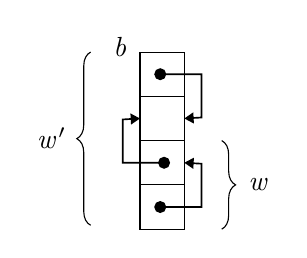
\begin{tikzpicture}[node distance=5mm]
    \node[pricell=$\vb$] (n1) {};
    \node[mpricell] (n2) [below=0pt of n1] {};
    \node[mpricell] (n3) [below=0pt of n2] {};
    \node[mpricell] (n4) [below=0pt of n3] {};
    \draw[ptr] (n1.center) to ++(0.5,0) to ++(0,-0.55) to (n2.east);
    \draw[ptr] (n3.center) to ++(-0.5,0) to ++(0,0.55) to (n2.west);
    \draw[ptr] (n4.center) to ++(0.5,0) to ++(0,0.55) to (n3.east);
    \draw[brace] (n3.north) to node[labbrace,yshift=-0.1em]{$\vw$} (n4.south);
    \draw[mbrace] (n1.north) to ++\south to node[lambrace,yshift=-0.75em]{$\vw'$} ++\south to++\south to ++\south;
\end{tikzpicture}
\end{center}

The End relation says that the component $\vf$ at world $\vw'$ and heap $\vh$ is completely determined by $\vf$ at $\vw' \setminus \{ \vb \}$ together with $\vh$ without cell $\vb$.
It is then clear to see that \countFun satisfies the End relation as it traverses the heap \emph{starting} from location $\va$.



\section{FGLS Monad on [Ctx,Set]}
\label{sec:fgls-ctx}

There is an inclusion functor $\vJ : \worldC \inclto \ctxC$ which by precomposition extends to a functor $\vJ^* : \funC\ctxC\setC \to \funC\worldC\setC$ and further an adjunction
\begin{tikzcd}
    {\funC\ctxC\setC} \arrow[rr, "\vJ^*", shift left=3] & \perp & {\funC\worldC\setC} \arrow[ll, "\vJ_*", shift left=3]
\end{tikzcd}
by taking the right Kan extension along $\vJ$.
The idea behind $\vJ_*$ is that while locations $\vl_1, \vl_2$ in $\worldC$ represent distinct locations, variables $\va, \vb$ in $\ctxC$ represent non-distinct aliases to locations.
To recover this aliasing, $\vJ_*$ considers all the possible ways this aliasing can happen.
                                
The $\vJ_* \vdash \vJ_*$ adjunction gives us a way to extend the full-ground monad $\monFLS$ to $\ctxC$ presheaves as:
    \[ \vX \mapsto \vJ_* (\monFLS(\vX\vJ)) : \funC\ctxC\setC \to \funC\ctxC\setC \]

\noindent
We shall now give an explicit definition of this monad using the following theorem:
\begin{theorem}\label{thm:ran-coslice-ends}
    Let $\vF : \mcatC \to \mcatD, \vA,\vB : \mcatC \to \setC$.
    We will show that:
        \[ \Ran\vF{\Exp\vB\vA}(\vD) \iso \End{\vf : \vD \to \vF\vC \in \commaC\vD\vF} \Exp{\vB\vC}{\vA\vC} \]
\end{theorem}
\begin{proof}
\begin{align*}
    \Ran\vF{\Exp\vB\vA}(\vD) \iso & \End{\vC \in \mcatC} \homF\mcatD\vD{\vF\vC} \to \Exp\vB\vA\vC        & \tag{\text{\cite{kelly2022basic} 4.24}} \\
                             \iso & \End{\vf : \vD \to \vF\vC \in \commaC\vD\vF} \Exp\vB\vA\vC         & \tag{\cref{adx:coslice-ends-proof}} \\
                             \iso & \End{\vf : \vD \to \vF\vC \in \commaC\vD\vF} \Exp{\vB\vC}{\vA\vC}  & \tag{\cref{adx:coslice-end-exponent-proof}}
\end{align*}
\end{proof}

\paragraph{The Monad}

Notice that:
\[ \vJ_* (\monFLS(\vX\vJ)) = \vJ_*\vU_*(\Exp{\vP(\vX\vJ\vU)}\heapF) = \Ran{\vJ\vU}{(\Exp{\vP(\vX\vJ\vU)}\heapF)} \]
We express the FGLS monad on $\funC\ctxC\setC$ using this observation and \cref{thm:ran-coslice-ends} as:

\[\begin{array}{rcl}
    \monFLSCtx & : & \funC\ctxC\setC \to \funC\ctxC\setC \\
    \monFLSCtx\vX & \eqdef & \End{\rho : \vw \to \vw' \in \commaC\vw{\vJ\vU}} \heapF\vw' \to \Coend{\rho' : \vw' \to \vw'' \in \commaC{\vw'}\vU} (\vX\vJ\vU)(\vw'') \times \heapF\vw''
\end{array}\]

\begin{theorem}
    The $\monFLSCtx$ monad is non-finitary.
\end{theorem}
\begin{proof}
    Follows directly from the non-finitary proof of $\monFLS$.
\end{proof}

\paragraph{Naturality-style}
\label{sec:fgls-ctx-natural}

We can give an alternative description of $\monFLSCtx$ using natural transformations by observing the action of the End.
Intuitively, its action is that every $\vf_{\rho_2}$ computation can be factored through a computation $\vf_{\rho_1}$ that requires a smaller starting heap followed by an extension of the result in a compatible way.
This forbids $\vf$ from using locations that are not \emph{reachable} from $\vw$ while at the same time allowing it to be called in all compatible future worlds.

Recall that the End quantifies over all morphisms $\rho : \vw \to \vw'$, and thus gives an $\rho$-ary product: 
\[ \phi \in \Prod{\vw \xto\rho \vw' \in \objC{\commaC\vw{\vJ\vU}}} \heapF\vw' \to \vP(\vX\vJ\vU \times \heapF)\vw' \]
such that the following coherence condition holds:

for every initialisation of the form:
 \begin{tikzcd} & {\vw} \arrow[dl, "\rho_1"'] \arrow[dr, "\rho_2"] & \\ 
               {\vw_1} \arrow[rr, "\vJ\vU\varepsilon"] && {\vw_2} 
 \end{tikzcd} and heap $\vh : \heapF\vw_1$
we have: \[\vP(\vX\vJ\vU\times\heapF)(\varepsilon)(\phi_{\rho_1}(\vh)) = \phi_{\rho_2}(\heapF(\varepsilon)\vh)\]

\noindent
 If we compare this data with the data of the following natural tranformations we see that they are isomorphic:
\[\begin{array}{c}
 \End{\rho : \vw \to \vw' \in \commaC\vw{\vJ\vU}}\heapF\vw' \to \vP(\vX\vJ\vU \times \heapF)\vw' \iso
    \homF{\funC\initC\setC}{\homF\ctxC\vw{\vJ\vU(\dash)} \times \heapF}{\vP(\vX\vJ\vU \times \heapF)}
\end{array}\]

We can go further and define the functorial action, unit and join of the FGLS monad in terms of this naturality style
which will be used in \cref{sec:finitary-monad} to define the finitary monad.

\paragraph{Functorial action}

\[\begin{array}{r@{\,}c@{\,}l}
    \monFLSCtx\vX(\vf : \vw \to \vw') & : & \monFLSCtx\vX\vw \to \monFLSCtx\vX\vw' \\
    \phi & \mapsto &  \homF\ctxC{\vw'}{\vJ\vU(\dash)} \times \heapF \xto{(\dash \comp \vf) \times 1} 
                      \homF\ctxC\vw{\vJ\vU(\dash)} \times \heapF \xto\phi \vP(\vX\vJ\vU \times \heapF)
\end{array}\]

\paragraph{Unit of Monad}

\[\begin{array}{r@{\,}c@{\,}l}
    \eta_\vX & : & \vX \To \monFLSCtx\vX \\
    \vx : \vX\vw & \mapsto & \homF\ctxC\vw{\vJ\vU(\dash)} \times \heapF \xto{\vX(\dash)(\vx) \times 1} \vX\vJ\vU \times \heapF 
                                                                                          \xto{\eta^\vP_{\vX\vJ\vU \times \heapF}} \vP(\vX\vJ\vU \times \heapF)
\end{array}\]

where $\vX(\dash)(\vx) : \homF\ctxC\vw{\vJ\vU(\dash)} \To \vX\vJ\vU$ is defined as $\vf \mapsto \vX(\vf)(\vx)$.

\paragraph{Join of Monad}

\[\begin{array}{r@{\,}c@{\,}l}
    \mu_\vX & : & \Exp\monFLSCtx2\vX \to \monFLSCtx\vX \\
    \phi & \mapsto & \homF\ctxC\vw{\vJ\vU(\dash)} \times \heapF \xto\phi \vP(\monFLSCtx\vX\vJ\vU \times \heapF) \xto{\vP(\eval)} \Exp\vP2(\vX\vJ\vU \times \heapF)
    \xto{\mu^\vP_{\vX\vJ\vU \times \heapF}} \vP(\vX\vJ\vU \times \heapF)
\end{array}\]

where $\eval : (\monFLSCtx\vX)\vJ\vU \times \heapF \To \vP(\vX\vJ\vU \times \heapF)$ is defined as $\tup\phi\vh_\vw \mapsto \phi_\vw\tup{1_\vw}\vh$.



\section{Becoming Finitary}

A natural question to ask is how to carve out a subset of the function space described by the FGLS monad such that the monad it induces is finitary.
Our goal is to prove a representation result between this finitary monad and the parametrised algebraic theory for FGLS.
Since the PAT for FGLS has models in $\funC\ctxC\setC$, we consider the finitary version of the FGLS monad lifted to $\ctxC$ presheaves (see \cref{sec:fgls-ctx}). 

\subsection{Preliminaries}

We first introduce some properties and constructions that are used to describe the finitary monad.

\subsubsection{Heaplet Initialisation Category}
The heaplet initialisation category $\dinitC$ is defined as:
\begin{itemize}
    \item Objects: Sort-preserving injective renamings between worlds $\vw^- \injto \vw^+$.
    \item Morphisms: Injective sort-preserving $\varepsilon^-$, sort-preserving $\varepsilon^+$, and a $\vh_\varepsilon : \dheapF(\vw_2^- \ominus \varepsilon^-, \vw_2^+)$ such that: 
                    \begin{center}
                     \begin{tikzcd}{\vw_1^+} \arrow[r, "{\varepsilon^+}"] & {\vw_2^+} \\
                                   {\vw_1^-} \arrow[u, tail, "\rho"] \arrow[r, tail, "{\varepsilon^-}"'] & {\vw_2^-} \arrow[u, tail, "\sigma"']
                     \end{tikzcd} 
                    \end{center}
\end{itemize}
We have functors $\vU_1 : \dinitC \to \worldC, \vU_2 : \dinitC \to \ctxC$ that project the first and second world correspondingly, 
$\initInclF : \initC \inclto \dinitC$ which maps $\vw$ to the corresponding identity morphism, and the heaplet functor can be defined as $\dheapF : \dinitC \to \setC$ 
(notice that we consider the heaplet functor to be of the form $\opC\worldC \times \ctxC \to \setC$).

\paragraph{An order on morphisms}

We say that a morphism $\varepsilon_2$ is \emph{at least as concrete} as $\varepsilon_2$ (notation $\varepsilon_1 \leq \varepsilon_2$), 
when $\varepsilon_1, \varepsilon_2$ have the same domain: 
\begin{center}
    \begin{tikzcd}
        {\vw_2^+} & {\vw^+} \arrow[l, "{\vU_2\varepsilon_2}"'] \arrow[r, "{\vU_2\varepsilon_1}"] & {\vw_1^+} \\
        {\vw_2^-} \arrow[u, tail] & {\vw^-} \arrow[u, tail, "{\rho}"] \arrow[l, tail, "{\vU_1\varepsilon_2}"] \arrow[r, tail, "{\vU_1\varepsilon_1}"'] & {\vw_1^-} \arrow[u, tail]
    \end{tikzcd} 
\end{center}
and satisfy:
\[ \text{ every } \vx \in \mathsf{Img}_{\vU_2\varepsilon_2}[\mathsf{Fibers}_{\vU_2\varepsilon_1}[\vw_1^+]] \text{ is a singleton set } \]
The idea is that $\varepsilon_2$ does not relate more dangling pointers from $\vw^+ \ominus \rho$ than $\varepsilon_1$.

\begin{example}
\end{example}

\begin{lemma}$\leq$ forms a preorder\end{lemma}

\paragraph{Extension Functor}
We define the extension functor as a means to add $\vw'$-many dangling pointers.
\[\begin{array}{r@{\,}c@{\,}l}
    \extF\dash{\vw'} & : & \dinitC \to \dinitC \\
    \extF{(\vw^- \xto\rho \vw^+)}{\vw'} & = & \vw^- \xto\rho \vw^+ \xinclto{\inl} \vw^+ \oplus \vw' \\
    \extF\varepsilon{\vw'} & = & \triple{\vU_1\varepsilon}{\vU_2\varepsilon \oplus 1_{\vw'}}{\dheapF\tup1\inl(\eta_\varepsilon)}
\end{array}\]
Further, for every functor $\vG : \dinitC \to \setC$, we have:
\[\begin{array}{r@{\,}c@{\,}l}
    \extNat\vG{\vw'} & : & \vG \To \vG\extF\dash{\vw'} \\
    \extNat\vG{\vw'}{(\vw^- \xto\rho \vw^+)} & = & \vG{\triple{1_{\vw^-}}{\inl^{\vw^+ \xinclto\inl \vw^+ \oplus \vw'}}\emptyset}
\end{array}\]
We will often drop $\vG$ from $\extNat\vG{\vw'}$ when it is clear from the context.

\subsubsection{Templates}

We introduce the notion of a \emph{template} that represents a collection of objects in $\dinitC$.
Specifically, a template is a set $\vI$ seen as a discrete category, together with a functor $\vT : \vI \to \dinitC$.
We say that a template is finite when $\vI$ is a finite set.

We would like to represent all the possible heap extensions that can be derived from a template.
For a template $\vT$, its heap extensions are given by the following functor:
\[\begin{array}{r@{\,}c@{\,}l}
    \templateExt\vF & : & \initC \to \setC \\
    \templateExt\vF & = & \colimit(\vI \xrightarrow\vT \dinitC \xrightarrow\vy \funC\dinitC\setC \xrightarrow{(\dash)\initInclF} \funC\initC\setC)
                                    \iso \Coprod{\vi \in \vI} \homF\dinitC{\vT(\vi)}{\initInclF(\dash)}
\end{array}\]

\subsubsection{Stencils}

Stencils are used to represent heaps with a common segment.
It is parametrised over a world $\vw$ that represents the public locations, and it is defined using heaplets with dangling pointers. 
Dangling pointers represent the points by which the stencil can be extended into a bigger heaplet/heap.

\[\begin{array}{r@{\,}c@{\,}l}
    \stencilF\nop & : & \opC\ctxC \to \funC\dinitC\setC \\
    \stencilF\vw & = & \homF\ctxC\vw{\vU_2(\dash)} \times \dheapF \\
    \stencilF\vf\tup\vg\vh & = & \tup{\vg \comp \vf}\vh
\end{array}\]

\begin{example}\label{exam:one}

Consider the following stencil given diagrammatically and assume all locations are of a single sort $\vC$
(locations in blue are directly accessible from the public world $\vw = \va$, pointers in red are dangling):
\begin{center}
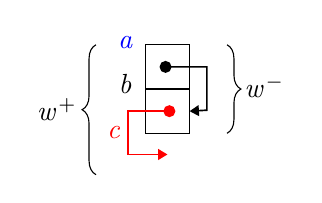
\begin{tikzpicture}[node distance=5mm]
    \node[pubcell=$\va$] (na) {};
    \node[pricell=$\vb$] (nb) [below=0pt of na] {};
    \draw[ptr] (na.center) to ++\east to ++\south to (nb.east);
    \draw[dptr] (nb.center) to ++\west  to node[midway,xshift=-0.5em] {$\vc$} ++\south to ++\east ;
    \draw[brace] (na.north) to node[labbrace]{$\vw^-$} (nb.south);
    \draw[mbrace] (na.north) to ++\south to node[lambrace]{$\vw^+$} ++\south to ++\south ;
\end{tikzpicture}
\end{center}
This stencil represents the heaps that have this segment as starting point from $\va$, to draw a few:
\begin{center}
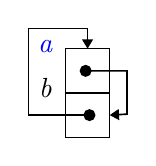
\begin{tikzpicture}[node distance=5mm]
    \node[pubcell=$\va$] (na) {};
    \node[pricell=$\vb$] (nb) [below=0pt of na] {};
    \draw[ptr] (na.center) to ++\east to ++\south to (nb.east);
    \draw[ptr] (nb.center) to ++\wwest to ++\north to ++\north to ++\eeast to (na.north);
\end{tikzpicture}
\hspace{2em}
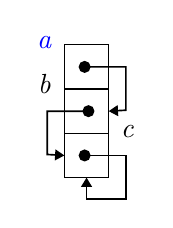
\begin{tikzpicture}[node distance=5mm]
    \node[pubcell=$\va$] (na) {};
    \node[pricell=$\vb$] (nb) [below=0pt of na] {};
    \node[mpricell=$\vc$] (nc) [below=0pt of nb] {};
    \draw[ptr] (na.center) to ++\east to ++\south to (nb.east);
    \draw[ptr] (nb.center) to ++\west to ++\south to (nc.west);
    \draw[ptr] (nc.center) to ++\east to ++\south to ++\west to (nc.south);
\end{tikzpicture}
\hspace{2em}
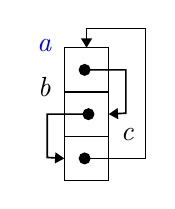
\begin{tikzpicture}[node distance=5mm]
    \node[pubcell=$\va$] (na) {};
    \node[pricell=$\vb$] (nb) [below=0pt of na] {};
    \node[mpricell=$\vc$] (nc) [below=0pt of nb] {};
    \draw[ptr] (na.center) to ++\east to ++\south to (nb.east);
    \draw[ptr] (nb.center) to ++\west to ++\south to (nc.west);
    \draw[ptr] (nc.center) to ++\eeast to ++\north to ++\north to ++\north to ++\wwest to (na.north);
\end{tikzpicture}
\end{center}
\end{example}

\paragraph{Rebasing a Stencil}

We define a covariant action of morphisms $\ctxC$ acting on a stencil which we call $\emph{rebasing}$.
For every morphism $\vf : \vw \to \vw' \in \ctxC$:
\[\begin{array}{r@{\,}c@{\,}l}
    \stencilRebase\vf & : & \stencilF\vw\extF\dash{\vw' \ominus \vf} \To \stencilF{\vw'}\extF\dash{\vw' \ominus \vf} \\
    \stencilRebase\vf_{\vw^- \xto\rho \vw^+}\tup{\vg^{\vw \to \vw^+ \oplus \vw' \ominus \vf}}\vh & \mapsto &
    \tup{\vw' \xto\iso \vw \oplus \vw' \ominus \vf \xto{[\vg,\inr]} \vw^+ \oplus \vw' \ominus \vf}\vh
\end{array}\]
\begin{lemma}\label{lem:stencilFretract}
The functorial action $\stencilF\vf$ is the retraction of the rebasing operation, that is:
\[ {\stencilF\vf}_{\extF\dash{\vw' \ominus \vf}} \comp \stencilRebase\vf = 1 \]
\end{lemma}

\begin{example}
    Consider the following extension $\vw = \va : \vC, \vw' = \va : \vC, \vd : \vC'$ and $\vf = \inl$. 
    We have that $\vw' \ominus \vf = \vd : \vC'$. 
    Consider a stencil that has $\vd$ as dangling reference:
    \[\begin{array}[t]{lll}
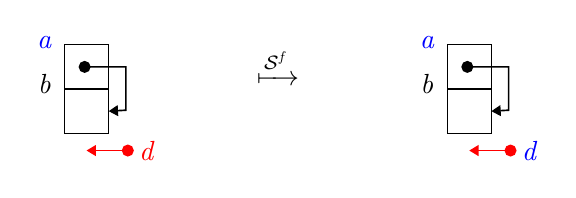
\begin{tikzpicture}[node distance=5mm]
    \node[pubcell=$\va$] (na) {};
    \node[pricell=$\vb$] (nb) [below=0pt of na] {};
    \draw[ptr] (na.center) to ++\east to ++\south to (nb.east);
    \draw[dptr] ($ (nb.center) + (0.5,-0.5) $) to node[midway,xshift=1.5em] {$\vd$} ++\west; 
    \node[draw=none] (nmap) [right=50pt of na.east] {$\xmapsto{\stencilRebase\vf}$};
    \node[pubcell=$\va$] (na2) [right=50pt of nmap] {};
    \node[pricell=$\vb$] (nb2) [below=0pt of na2] {};
    \draw[ptr] (na2.center) to ++\east to ++\south to (nb2.east);
    \draw[dptr] ($ (nb2.center) + (0.5,-0.5) $) to node[midway,xshift=1.5em,color=blue] {$\vd$} ++\west; 
\end{tikzpicture}
\end{array}\]
    The rebasing operation simply makes the location $\vd$ publicly accessible from $\vw'$. 
\end{example}

\subsubsection{Stencil Cover}

We view stencils accessible via a world $\vw$ as a category by considering the category of elements for functor $\stencilF\vw$ \ie $\coeC{\stencilF\vw}$,
defined as:
\begin{itemize}
    \item Objects: $\tup{\rho : \vw^- \injto \vw^+}{\vs \in \stencilF\vw(\rho)}$
    \item Morphisms: $\tup{\rho}\vs \xrightarrow\varepsilon \tup{\sigma}{\vs'}$
                    is a morphism $\varepsilon : \rho \to \sigma \in \dinitC$, such that $\stencilF\vw(\varepsilon)(\vs) = \vs'$
\end{itemize}

A \emph{stencil cover} is a collection of stencils that is compatible with a particular template.
That is, a $\vw$-accessible $\vT$-cover, is a functor $\vS : \vI \to \coeC{\stencilF\vw}$ such that:
\begin{center}
\begin{tikzcd}
    {\vI} \arrow[rr, "{\vT}"] \arrow[dr, "{\vS}"'] && {\dinitC} \\
        & {\coeC{\stencilF\vw}} \arrow[ur, "{\vU}"'] &
\end{tikzcd}
\end{center}
We have a natural transformation $\cov : \templateExt\vT \To \homF\ctxC\vw{\vJ\vU(\dash)} \times \heapF$ given by:
\[ \tup\vi{\varepsilon^{\vT(\vi) \to \sigma}} \mapsto \stencilF\vw(\varepsilon)(\projTwo(\vS\vi)) \]
We say that a cover is \emph{complete} when $\cov$ is an isomorphism.

\subsubsection{Heaplet Hiding Monad}
We further generalise the hiding monad to heaplets as follows (see \cref{adx:heaplet-hiding-mon} for the functorial action):
\[\begin{array}{r@{\,}@{\,}l@{\,}l@{\,}}
    \dhideMon          :&\multicolumn{2}{l}{\funC\dinitC\setC \to \funC\dinitC\setC} \\
    (\dhideMon\vA)(\rho : \vw^- \injto \vw^+)  =& \Coend{\vw^- \injto \vw' \in \commaC{\vw^-}\vU} 
                                                             \vA(\inl^{\vw' \inclto \vw' \oplus \vw^+ \ominus \rho})
\end{array}\]
which takes the coend of $\opC{(\commaC{\vw^-}\vU)} \times \commaC{\vw^-}\vU \xrightarrow\projTwo \commaC{\vw^-}\vU \xrightarrow\vU \initC \xrightarrow{\initInclF} \dinitC  \xrightarrow{\extF\dash{\vw^+ \ominus \rho}} \dinitC \xrightarrow\vA \setC$.
We have a natural isomorphism $\dhideMon(\vX \odot \dheapF)\initInclF \iso \hideMon(\vX \odot \heapF)$
between the hiding monad on heaplets with the one on heaps when $\vA = \vX \odot \dheapF$.

We consider the action of $\dhideMon\vA$ on morphisms as consisting of two parts: 
\begin{itemize}
    \item An action between elements of the equivalence classes (does not satisfy functoriality): 
        \[ \dhideMonSk\vA(\varepsilon : \rho \to \sigma) : \Coprod{\vw_1^- \injto \vw'} \vA(\inl^{\vw' \to \vw' \oplus (\vw_1^+ \ominus \rho)}) \to
                                                           \Coprod{\vw_2^- \injto \vw'} \vA(\inl^{\vw' \to \vw' \oplus (\vw_2^+ \ominus \sigma)}) \]
    \item A quotienting step given by the coend to make it functorial: 
            \[ \dhideMon\vA(\varepsilon)(\quot{\rho'}\va) = [\underline{\mathbb{P}}\vA(\varepsilon)(\inj{\rho'}\va)] \]
\end{itemize}
We further consider a variation of the category of elements for $\dhideMon\vA$ that will circumvent the need for representatives in later constructions.
Define the category of elements $\maxC{\dhideMonSk\vA}$, as follows:
\begin{itemize}
    \item Objects: $\tup{\rho \in \dinitC}{\vp \in \dhideMonSk\vA(\rho)}$
    \item Morphisms: $\tup\rho\vp \to \tup\sigma\vs$ is a morphism $\varepsilon : \rho \to \sigma \in \dinitC$ such that $\dhideMon\vA(\varepsilon)[\vp] = [\vs]$
\end{itemize}
Thus the objects of this category are the elements of the equivalence classes of $\dhideMon\vA$ and not the equivalence classes themselves.

\subsubsection{Evaluations}

We associate a template with its evaluations using the above hiding monad as the codomain. 
Define an $\vX$-valued $\vT$-evaluation as a functor $\vE : \vI \to \maxC{\dhideMonSk(\vX \odot \dheapF)}$ that is compatible with $\vT$:
\begin{center}
\begin{tikzcd}
    {\vI} \arrow[rr, "{\vT}"] \arrow[dr, "{\vE}"'] && {\dinitC} \\
        & {\maxC{\dhideMonSk(\vX \odot \dheapF)}} \arrow[ur, "{\vU}"'] &
\end{tikzcd}
\end{center}
We have a natural transformation $\ev : \templateExt\vT \To \hideMon(\vX \odot \heapF)$ given by:
\[ \tup\vi{\varepsilon^{\vT(\vi) \to \sigma}} \mapsto \iso^{\dhideMon(\vX \odot \dheapF)\initInclF, \hideMon(\vX \odot \heapF)}(\dhideMon(\vX \odot \dheapF)(\varepsilon)[\projTwo(\vE\vi)] \]

\subsection{Finitary Monad}
\label{sec:finitary-monad}

A $\phi \in (\monFLSCtx\vX)\vw$ is finitary when it is generated by its actions on a finite number of \emph{heaplets}. 

\[\begin{array}{r@{\,\,}l@{\,}l@{\,}}
    \monFLSfin         : &\multicolumn{2}{l}{\funC\ctxC\setC \to \funC\ctxC\setC} \\
    (\monFLSfin\vX)\vw =& \{ \phi \in (\monFLSCtx\vX)\vw :& \textit{exists a finite template $\vT$,} \\
                        &&                                  \textit{a complete $\vw$-accessible $\vT$-cover $\vS$,} \\ 
                        &&                                  \textit{an $\vX$-valued $\vT$-evaluation $\vE$,} \\
                        &&                                  \textit{such that $\ev_\vE \comp \cov_\vS^{-1} = \phi$} \}
\end{array}\]

\begin{itemize}
    \item We consider $\phi \in (\monFLSCtx\vX)\vw$ using its naturality description (see \cref{sec:fgls-ctx-natural}).
    \item We require a finite template, and thus we have a finite number of stencils.
    \item We require a complete cover, so $\cov : \templateExt\vF \To \homF\ctxC\vw{\vU(\dash)} \times \heapF$ is an isomorphism.
          This gives us that every $\tup\vf\vh$ is mapped to exactly one stencil $\vS\vi$ and morphism $\varepsilon$ such that $\stencilF\vw(\varepsilon)(\projTwo(\vS\vi)) = \tup\vf\vh$.
      \item We require that morphism $\phi$ lifts through $\cov^{-1}$ using the morphism $\ev$ induced by the evaluation $\vE$.
          This means that the following diagram commutes:
          \begin{center}
            \begin{tikzcd}
                {\homF\ctxC\vw{\vJ\vU(\dash)} \times \heapF} \arrow[rr, "{\phi}"] \arrow[rd, "{\cov^{-1}}"'] && {\hideMon(\vX \odot \heapF)} \\
                                                                                    & {\templateExt\vT} \arrow[ur, "{\ev}"']
            \end{tikzcd}
          \end{center}
\end{itemize}

\subsubsection{Action on Morphisms}

We show that the factorial action of the $\monFLSfin$ monad on morphisms lifts through $\monFLSCtx$, that is, for every $\vf : \vw \to \vw'$ we have functor $\vG : \vI' \to \commaC\vy{\stencilF{\vw'}}$ and morphism $\vh$ such that: 
\begin{center}
\begin{tikzcd}
    {\homF\ctxC{\vw'}{\vJ\vU\dash}} \arrow[d, "{\iso}"] \arrow[rr, "{(\dash \comp \vf) \times 1}"] && 
    {\homF\ctxC\vw{\vJ\vU\dash}}    \arrow[r, "{\phi}"] \arrow[d, "{\iso}"]   & {\hideMon(\vX\vJ\vU \times \heapF)} 
\\
    {\templateExt{\vG}\initInclF} \arrow[rr, "{\vh_{\initInclF(\dash)}}"'] \arrow[u, "{\cov{\initInclF(\dash)}}"] &&
    {\templateExt\vF\initInclF} \arrow[u, "{\cov{\initInclF(\dash)}}"] \arrow[ur, "{\ev{\initInclF(\dash)}}"']
\end{tikzcd}
\end{center}

\begin{proof}
We utilize the structure of the functorial action on morphisms, that is,
for a morphism $\varepsilon : \rho \to \sigma$, $\inj{\rho'}\va$, $\dhideMon\vA(\varepsilon)[\inj{\rho'}\va]$ will give a 

Every morphism $\vf : \vw \to \vw' \in \ctxC$ induces a functor $\rebaseF\vf : \coeC{\stencilF\vw} \to \coeC{\stencilF{\vw'}}$
which extends a stencil with $\vw' \ominus \vf$ pointers and then rebases it: 
\[\begin{array}{r@{\,}c@{\,}l}
    \rebaseF\vf & : & \coeC{\stencilF\vw} \to \coeC{\stencilF{\vw'}} \\
    \tup\rho\vs & \mapsto & \tup{\extFNB\rho{(\vw' \ominus \vf)}}{\stencilRebase\vf(\extNat\nop{\vw' \ominus \vf}(\vs))} \\
    \varepsilon & \mapsto & \extFNB\varepsilon{(\vw' \ominus \vf)}
\end{array}\]

\begin{example}
    Consider the stencil from \cref{exam:one} and the extension of $\vw = \va : \vC$ to $\vw' = \va : \vC, \vd : \vC'$.
    The resulting stencil has an extra dangling pointer $\vd : \vC'$ and so any extension of the stencil must be a heap that is defined with a location of sort $\vC'$. 
\begin{center}
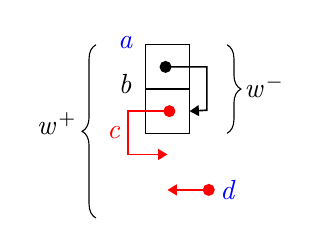
\begin{tikzpicture}[node distance=5mm]
    \node[pubcell=$\va$] (na) {};
    \node[pricell=$\vb$] (nb) [below=0pt of na] {};
    \draw[ptr] (na.center) to ++\east to ++\south to (nb.east);
    \draw[dptr] (nb.center) to ++\west to node[midway,xshift=-0.5em] {$\vc$} ++\south to ++\east;
    \draw[dptr] ($ (nb.center) + (0.5,-1) $) to node[midway,xshift=1.5em,color=blue] {$\vd$} ++\west; 
    \draw[brace] (na.north) to node[labbrace]{$\vw^-$} (nb.south);
    \draw[mbrace] (na.north) to ++\south to node[lambrace,yshift=-0.5em]{$\vw^+$} ++\south to ++\south to ++\south;
\end{tikzpicture}
\end{center}
\end{example}

    Consider $\vG = \rebaseF\vf\vF : \vI \to \commaC\vy{\stencilF{\vw'}}$ and $\vh = \coprod{\vy\tup1\inl}$.
\begin{center}
\begin{tikzcd}
    {\homF\ctxC{\vw'}{\vJ\vU\dash}} \arrow[d, "{\iso}"] \arrow[r, "{(\dash \comp \vf) \times 1}"] & 
    {\homF\ctxC\vw{\vJ\vU\dash}}    \arrow[r, "{\phi}"] \arrow[d, "{\iso}"]   & {\hideMon(\vX\vJ\vU \times \heapF)} 
\\
    {\templateExt{(\rebaseF\vf\vF)}\initInclF} \arrow[r, "{\coprod{\vy\tup1\inl}_{\initInclF(\dash)}}"'] \arrow[u, "{\cov{\initInclF(\dash)}}"] & 
    {\templateExt\vF\initInclF} \arrow[u, "{\actV\phi{\initInclF(\dash)}}"] \arrow[ur, "{\resV\phi{\initInclF(\dash)}}"']
\end{tikzcd}
\end{center}

That $\cov{\initInclF(\dash)}$ is iso and that the square commutes follows from \cref{lem:stencilFretract} by observing that:
\begin{center}
\begin{tikzcd}
    {\homF\ctxC{\vw'}{\vJ\vU\dash}} \arrow[d, "{\iso}"] \arrow[rr, "{(\dash \comp \vf) \times 1}"] && {\homF\ctxC\vw{\vJ\vU\dash}} \arrow[d, "{\iso}"] \\
    {\stencilF{\vw'}\initInclF} \arrow[u] \arrow[rr, "{\stencilF\vf}"] && {\stencilF\vw\initInclF} \arrow[u]
\end{tikzcd}
\end{center}
\orpheas{TODO: Latexify the handwritten proof.}
Further, every $\vf : \vw \to \vw'$ induces a natural transformation $\coprod{\vy\tup1\inl} : \templateExt{(\rebaseF\vf \comp \vF)} \To \templateExt\vF$:
\[    \tup\vi{\varepsilon^{\extF{\vU\vF(\vi)}{\vw' \ominus \vf} \to \sigma}} \mapsto \tup\vi{\varepsilon \comp \triple{1}{\inl}\emptyset} \]

\end{proof}

\subsubsection{Unit of Monad}

We show that the unit of the $\monFLSfin$ monad lifts through $\monFLSCtx$, that is, $\eta_{\vX,\vw}(\vx)$ satisfies: 
\begin{center}
\begin{tikzcd}
    {\homF\ctxC\vw{\vJ\vU(\dash)} \times \heapF} \arrow[d, "{\iso}"] \arrow[rrr, "{\eta^\vP \comp \vX(\dash)(\vx) \times 1}"] &&& {\vP(\vX\vJ\vU \times \heapF)} 
\\
    {\templateExt\vF\initInclF} \arrow[u, "{\cov{\initInclF(\dash)}}"] \arrow[urrr, "{\ev{\initInclF(\dash)}}"']
\end{tikzcd}
\end{center}
\begin{proof}
    Consider the stencil $\vs = \tup{1_\vw}\emptyset : \stencilF\vw(\emptyset \injto \vw)$ that has only $\vw$ dangling pointers, and let $\vF(*) = \vs : 1 \to \commaC\vy{\stencilF\vw}$.
    That $\cov{\initInclF(\dash)}$ is iso is given by $\tup\vf\vh \mapsto \inj{*}{\triple{? : \emptyset \injto \vw}\vf\vh}$ and $\ev\nop$ is defined as:
    \[ \ev\nop(\inj{*}\varepsilon) = \dhideMon(\vX\vU_2 \times \dheapF)(\varepsilon)(\eta^{\dhideMon}_{\emptyset \to \vw}\tup{\vx}\emptyset) \]
\end{proof}

\subsubsection{Kleisli Extension of Monad}

\begin{center}
\begin{tikzcd}
    & {\rho} \arrow[d] \arrow[ld, "{\varepsilon_1}"'] \arrow[rd, "{\varepsilon_2}"] & \\
    {\rho_1} \arrow[rd, "{\hat{\varepsilon_1}}"'] & {\rho_\vr} \arrow[l, "{\varepsilon_1'}"'] \arrow[r, "{\varepsilon_2'}"] & {\rho_2} \arrow[ld, "{\hat{\varepsilon_2}}"] \\
                        & {\hat\rho} &
\end{tikzcd}
\end{center}
${\varepsilon_1 \oplus_{\rho} \varepsilon_2} :=$ Treat pointers from $\rho_1$, $\rho_2$ as distinct unless they come from the same domain and do this recursively by following the allocated data from $\varepsilon_1$, $\varepsilon_2$.

\[\begin{array}[t]{lll}
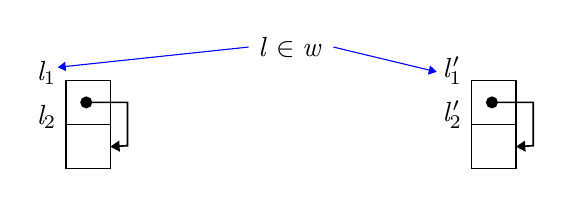
\begin{tikzpicture}[node distance=5mm]
    \node[pricell=$\vl_1$] (l1) {};
    \node[pricell=$\vl_2$] (l2) [below=0pt of l1] {};
    \draw[ptr] (l1.center) to ++\east to ++\south to (l2.east);

    \node[draw=none] (l) [right=50pt of l1.east, yshift=20pt] {$\vl \in \vw$};
    \draw[draw=blue, -{Triangle[scale=0.8]}, shorten >=-3pt] (l.west) to ([yshift=5]l1.north west); 

    \node[pricell=$\vl_1'$] (l1') [right=50pt of l, yshift=-20pt] {};
    \draw[draw=blue, -{Triangle[scale=0.8]}, shorten >=13pt] (l.east) to (l1'.north west);

    \node[pricell=$\vl_2'$] (l2') [below=0pt of l1'] {};
    \draw[ptr] (l1'.center) to ++\east to ++\south to (l2'.east);
\end{tikzpicture}
\end{array}\]

\paragraph{Reachable/Unreachable Factorisation System}

\def\reach{\mathsf{reach}}

The category $\dinitC$ has an orthogonal factorisation system $(\vE,\vM)$ that splits a morphism $\varepsilon : \rho_1 \to \rho_2$ into an $\ve : \rho_1 \to \rho_1^\reach$ representing the reachable part of $\eta_\varepsilon$ and $\vm : \rho_1^\reach \to \rho_2$ representing the rest unreachable part.

We can then define local independent morphisms $\vf, \vg$ as:

\begin{center}
\begin{tikzcd}
                       && {\rho} \arrow[lld, "{\varepsilon_1}"'] \arrow[ld, "{\ve_1}"] \arrow[rrd, "{\varepsilon_2}"] \arrow[rd, "{\ve_2}"'] && \\
    {\rho_1} \arrow[rrd, "{\vf}"'] & {\rho_1^\reach} \arrow[l, "{\vm_1}"'] & & {\rho_2^\reach} \arrow[r, "{\vm_2}"] & {\rho_2} \arrow[lld, "{\vg}"] \\
         && {\hat\rho} &&
\end{tikzcd}
\end{center}

\begin{center}
\begin{tikzcd}
                       && {\rho} \arrow[lld, "{\varepsilon_1}"'] \arrow[ld, "{\ve_1}"] \arrow[rrd, "{\varepsilon_2}"] \arrow[rd, "{\ve_2}"'] && \\
    {\rho_1} \arrow[rrd, "{\vf}"'] & {\rho_1^\reach} \arrow[l, "{\vm_1}"'] & & {\rho_2^\reach} \arrow[r, "{\vm_2}"] & {\rho_2} \arrow[lld, "{\vg}"] \\
         && {\hat\rho} &&
\end{tikzcd}
\end{center}
such that if $\vU^+(\vf)(\va) = \vU^+(\vg)(\vb)$ then $\va \in \img{\vU^+(\vm_1)}$ and $\vb \in \img{\vU^+(\vm_2)}$.

In words: if two pointers are related then they must come from the reachable part.

\appendix

\section{Appendix}

\subsection{Hiding Monad on Heaplets}
\label{adx:heaplet-hiding-mon}

Recall the action of $\dhideMon$ on objects:
\[\begin{array}{r@{\,}@{\,}l@{\,}l@{\,}}
    \dhideMon          &:&\funC\dinitC\setC \to \funC\dinitC\setC \\
    (\dhideMon\vA)(\rho : \vw^- \injto \vw^+)  &=& \Coend{\vw^- \injto \vw' \in \commaC{\vw^-}\vU} 
                                                             \vA(\vi^{\vw' \inclto \vw' \oplus \vw^+ \ominus \rho})
\end{array}\]
The action on morphism $\varepsilon = 
\begin{tikzcd}
    {\vw_1^+} \arrow[rr, "{\vU_2\varepsilon}"] && {\vw_2^+} \\
    {\vw_1^-} \arrow[u, "{\rho}"] \arrow[rr, "{\vU_1\varepsilon}"'] && {\vw_2^-} \arrow[u, "{\sigma}"'] \\
\end{tikzcd}, \vh_\varepsilon : \dheapF(\vw_2^- \ominus \vU_1\varepsilon, \vw_2^+)$ is given as:

\[\begin{array}{r@{\,}@{\,}l@{\,}l@{\,}}
    \dhideMon\vA(\varepsilon) &:& \dhideMon\vA\rho \to \dhideMon\vA\sigma \\
    \quot{\vw_1^- \xrightarrow{\rho'} \vw'}\va & \mapsto&
        \quot{\vw_2^- \xrightarrow{(\vU_1\varepsilon)^*\rho'} \rho' \oplus_{\vw_1^-} \vU_1\varepsilon}\vA(\varepsilon')(\va)
\end{array}\]

Where $(\vU_1\varepsilon)^*\rho'$ comes from:
\begin{tikzcd}
    {\vw_1^-} \arrow[d, "\rho'"'] \arrow[rr, "{\vU_1\varepsilon}"] && {\vw_2^-} \arrow[d, "{(\vU_1\varepsilon)^*\rho'}"] \\
    {\vw'} \arrow[rr, "{(\rho')^*\vU_1\varepsilon}"'] && {\rho' \oplus_{\vw_1^-} \vU_1\varepsilon}
\end{tikzcd}

and $\varepsilon'$ is:
\begin{tikzcd}
    {\vw' \oplus (\vw_1^+ \ominus \rho)} \arrow[rrr, "{[(\rho')^*\vU_1\varepsilon, \psi \comp \vU_2\varepsilon \comp \compl\rho]}"] &&& 
        {\rho' \oplus_{\vw_1^-} \vU_1\varepsilon \oplus \vw_2^+ \ominus \sigma} \\
    {\vw'} \arrow[u, hook] \arrow[rrr, "{(\rho')^*\vU_1\varepsilon}"] &&& 
        {\rho' \oplus_{\vw_1^-} \vU_1\varepsilon} \arrow[u, hook]
\end{tikzcd}, $\dheapF(\iso, \psi)(\eta_\varepsilon)$

where $\psi$ is given by: 
\[ \vw_2^+ \xrightarrow\iso \vw_1^- \oplus (\vw_2^- \ominus \vU_1\varepsilon) \oplus (\vw_2^+ \ominus \sigma)
           \inclto \rho' \oplus_{\vw_1^-} \vU_1\varepsilon \oplus \vw_2^+ \ominus \sigma
\]

We will often consider the action of $\dhideMon\vA(\varepsilon)$ as two parts: 
\begin{itemize}
    \item An action between elements of the equivalence classes (does not satisfy functoriality): 
        \[ \begin{array}{r@{\,}c@{\,}l}
            \dhideMonSk\vA(\varepsilon : \rho \to \sigma) & : & \Coprod{\vw_1^- \injto \vw'} \vA(\inl^{\vw' \to \vw' \oplus (\vw_1^+ \ominus \rho)}) \to
                                                                \Coprod{\vw_2^- \injto \vw'} \vA(\inl^{\vw' \to \vw' \oplus (\vw_2^+ \ominus \sigma)}) \\
            \dhideMonSk\vA(\varepsilon)(\inj{\rho'}\va) &  =  & \inj{\vU_1\varepsilon*\rho'}\vA(\varepsilon')(\va)
        \end{array}\]
    \item A quotienting step given by the coend to make it functorial: 
            \[ \dhideMon\vA(\varepsilon)(\quot{\rho'}\va) = [\underline{\mathbb{P}}\vA(\varepsilon)(\inj{\rho'}\va)] \]
\end{itemize}

% \subsection{Heaplet Compatibility}
% \label{adx:heaplet-compatibility}

% We say that $\tup{\vw \xrightarrow\rho \vw^- \xrightarrow{\rho^+} \vw^+}{\vh' : \dheapF(\vw^-,\vw^+)}$ is compatible with:
% \[ \tup{{\ubar\vw}^- \xrightarrow{\sigma^+} {\ubar\vw}^+ \xleftarrow\sigma \vw^+}{\ubar\vh : \dheapF(\ubar\vw^-, \ubar\vw^+)} \]
% when the following conditions are met:
% \begin{itemize}
%     \item For all their shared locations, $\vh'$ and $\ubar\vh$ store the same values, that is, we have:
%             \[ \dheapF(\nu_*, \sigma)(\vh') = \dheapF(\ext\nu, 1_{\ubar\vw^+})(\ubar\vh) \]

%         Where $\nu_*, \ext\nu$ come from the following pullback diagram:
%         \begin{center}
%             \begin{tikzcd}
%                 {\vv} \arrow[d, "{\nu_*}"'] \arrow[rr, "{\ext\nu}"] && {\ubar\vw^-} \arrow[d, "{\sigma^+}"] \\
%                 {\vw^-} \arrow[r, "{\rho^+}"] & {\vw^+} \arrow[r, "{\sigma}"] & {\ubar\vw^+} \\
%             \end{tikzcd}
%         \end{center}
%     \item The part of heap $\ubar\vh$ that is not shared with $\vh'$ does not have references to locations $\vw^- \ominus \rho$ (representing the newly allocated locations):

%           There exists a $\eta_{\varepsilon_1} : \dheapF(\ubar\vw^- \ominus \nu^*, \ubar\vw^+ \ominus \tau)$ where $\tau$ is:
%             \[ \vw^- \ominus \rho \xrightarrow{\compl\rho} \vw^- \xrightarrow{\rho^+} \vw^+ \xrightarrow\sigma \ubar\vw^+ \]
%           such that $\dheapF(1, \compl\tau)(\eta_{\varepsilon_1}) = \dheapF(\compl{\ext\nu}, 1)(\ubar\vh)$.
% \end{itemize}

% % The above data give us the following morphisms in $\dinitC$:
% % \[\begin{array}{lcr}
% %     \varepsilon_1 : 1_\vv \to \sigma^+ = \triple{\ext\nu}{\sigma^+ \comp \ext\nu}{\dheapF(1, \compl\tau)(\eta_{\varepsilon_1})} & \text{ and } &
% %     \varepsilon_2 : 1_\vv \to \rho^+ = \triple{\nu_*}{\rho^+ \comp \nu_*}{\dheapF(\compl{\nu_*}, 1)(\vh')}
% % \end{array}\]

% The above data give us the following heaplets:
% \[\begin{array}{lcr}
%     \eta_{\varepsilon_1} : \dheapF(\ubar\vw^- \ominus \nu^*, \ubar\vw^+ \ominus \tau) & \text{ and } &
%     \eta_{\varepsilon_2} = \dheapF(\compl{\nu_*}, 1)(\vh') : \dheapF(\vw^- \ominus \nu_*, \vw^+)
% \end{array}\]

\subsection{End related lemmas}
\label{adx:end-lemmas}

Unless otherwise specified let $\vA,\vB,\vG : \mcatC \to \setC$, $\vF : \mcatC \to \mcatD$  and the following morphisms in $\commaC\vD\vF$:
\begin{center}
\begin{tikzcd}
    {\vF\vC}
        \arrow[rr, "{\vF\vh}"]
    &&
    {\vF\vC'}
    \\
    &
    {\vD}
        \arrow[ul, "\vf"]
        \arrow[ur, "\vg"']
\end{tikzcd}
\end{center}

\begin{lemma}\label{adx:coslice-ends-proof}
    \[ \End{\vC \in \mcatC} \Exp{\vG\vC}{\homF\mcatD\vD{\vF\vC}} \iso \End{\vf : \vD \to \vF\vC \in \commaC\vD\vF} \vG\vC \]
\end{lemma}
\begin{proof}
    The morphism $\End{\vC \in \mcatC} \Exp{\vG\vC}{\homF\mcatD\vD{\vF\vC}} \dashrightarrow \End{\vf : \vD \to \vF\vC \in \commaC\vD\vF} \vG\vC$ is from the following wedge:
    \begin{center}
        \begin{tikzcd}
            & {\End{\vC \in \mcatC} \Exp{\vG\vC}{\homF\mcatD\vD{\vF\vC}}}
                \arrow[dl, "\proj\vC"']
                \arrow[dr, "\proj{\vC'}"]
        \\
            {\Exp{\vG\vC}{\homF\mcatD\vD{\vF\vC}}}
                \arrow[dd, "{\dash(\vf)}"]
                \arrow[dr, "{\vG\vh \comp \dash}"]
            &&
            {\Exp{\vG{\vC'}}{\homF\mcatD\vD{\vF{\vC'}}}}
                \arrow[dd, "{\dash(\vg)}"]
                \arrow[dl, "{\Lam\vk \dash(\vF\vh \comp \vk)}"']
        \\
            &
                {\Exp{\vG{\vC'}}{\homF\mcatD\vD{\vF\vC}}}
                    \arrow[dr, "{\dash(\vf)}"]
            &
        \\
            {\vG\vC}
                \arrow[rr, "{\vG\vh}"]
            &&
            {\vG{\vC'}}
        \end{tikzcd}
    \end{center}
    The morphism $\End{\vf : \vD \to \vF\vC \in \commaC\vD\vF} \vG\vC \dashrightarrow \End{\vC \in \mcatC} \Exp{\vG\vC}{\homF\mcatD\vD{\vF\vC}} $ is from the following wedge:
    \begin{center}
        \begin{tikzcd}
            &
                {\End{\vf : \vD \to \vF\vC \in \commaC\vD\vF} \vG\vC}
                    \arrow[dl, "{\Lam\vf \proj\vf(\dash)}"']
                    \arrow[dr, "{\Lam\vg \proj\vg(\dash)}"]
                    \arrow[dd, "{\Lam\vk \proj{\vF\vh \comp \vk}(\dash)}"]
        \\
            {\Exp{\vG\vC}{\homF\mcatD\vD{\vF\vC}}}
                \arrow[dr, "{\vG\vh \comp \dash}"]
            &&
            {\Exp{\vG{\vC'}}{\homF\mcatD\vD{\vF{\vC'}}}}
                \arrow[dl, "{\Lam\vk \dash(\vF\vh \comp \vk)}"]
        \\
            &
                {\Exp{\vG{\vC'}}{\homF\mcatD\vD{\vF\vC}}}
        \end{tikzcd}
    \end{center}
    It follows directly that these two induced morphisms are inverses, and thus the two ends are isomorphic.
\end{proof}

\begin{lemma}\label{adx:coslice-end-exponent-proof}
    \[ \End{\vf : \vD \to \vF\vC \in \commaC\vD\vF} \Exp\vB\vA\vC \iso \End{\vf : \vD \to \vF\vC \in \commaC\vD\vF} \Exp{\vB\vC}{\vA\vC} \]
\end{lemma}
\begin{proof}

The morphism  $\End{\vf : \vD \to \vF\vC \in \commaC\vD\vF} \Exp\vB\vA\vC \dashrightarrow \End{\vf : \vD \to \vF\vC \in \commaC\vD\vF} \Exp{\vB\vC}{\vA\vC}$ is from the following wedge:
\begin{center}
    \begin{tikzcd}
    & {\End{\vf : \vD \to \vF\vC \in \commaC\vD\vF} \Exp\vB\vA\vC}
        \arrow[dl, "{\proj\vf}"']
        \arrow[dr, "{\proj\vg}"]
    \\
    {\Exp\vB\vA\vC}
        \arrow[d, "{\Lam\va (\dash)_\vC\tup{1_\vC}\va}"]
        \arrow[rr, "{(\Lam{\tup\vk\va} (\dash)_{\hat\vC}\tup{\vk \comp \vh}\va)_{\hat\vC \in \mcatC}}"]
        &&
    {\Exp\vB\vA{\vC'}}
        \arrow[d, "{\Lam{\va'} (\dash)_{\vC'}\tup{1_{\vC'}}{\va'}}"]
    \\
    {\Exp{\vB\vC}{\vA\vC}}
        \arrow[dr, "{\vB\vh \comp \dash}"]
        &&
    {\Exp{\vB\vC'}{\vA\vC'}}
        \arrow[dl, "{\dash \comp \vA\vh}"]
    \\
    &
    {\Exp{\vB\vC'}{\vA\vC}}
    \end{tikzcd}
\end{center}

The morphism  $\End{\vf : \vD \to \vF\vC \in \commaC\vD\vF} \Exp{\vB\vC}{\vA\vC} \dashrightarrow \End{\vf : \vD \to \vF\vC \in \commaC\vD\vF} \Exp\vB\vA\vC$ is from the following wedge:
\begin{center}
    \begin{tikzcd}
        &
        {\End{\vf : \vD \to \vF\vC \in \commaC\vD\vF} \Exp{\vB\vC}{\vA\vC}}
            \arrow[dl, "{(\Lam{\tup\vk\va} \proj{\vF\vk \comp \vf} (\dash)(\va))_{\hat\vC \in \mcatC}}"']
            \arrow[dr, "{(\Lam{\tup\vk\va} \proj{\vF\vk \comp \vg} (\dash)(\va))_{\hat\vC \in \mcatC}}"]
    \\
        {\Exp\vB\vA\vC}
        \arrow[rr, "{\Exp\vB\vA\vh = (\Lam{\tup\vk\va} (\dash)_{\hat\vC}\tup{\vk \comp \vh}\va)_{\hat\vC \in \mcatC}}"']
    &&
        {\Exp\vB\vA{\vC'}}
    \end{tikzcd}
\end{center}
    which commutes by:
\begin{tikzcd}
    {\vF{\hat\vC}}
        \arrow[rr, no head, Rightarrow, no head]
    &&
    {\vF{\hat\vC}}
    \\
    {\vF{\vC'}}
        \arrow[u, "{\vF\vk}"]
    &&
    \\
    {\vF\vC}
        \arrow[u, "{\vF\vh}"]
        \arrow[rr, "{\vF\vh}"]
    &&
    {\vF\vC'}
        \arrow[uu, "{\vF\vk}"]
    \\
    &
    {\vD}
        \arrow[ul, "\vf"]
        \arrow[ur, "\vg"']
\end{tikzcd}
\end{proof}
\noindent
That the end projections form a natural transformation and that the two induced morphisms are inverses is not hard to prove.


\printbibliography

\end{document}
\endinput
